\documentclass{hw-template}

\newcommand{\V}{\mathbb{V}}
\newcommand{\W}{\mathbb{W}}

\title{NE523 Homework 1}
\author{Kyle Hansen}
\date{2 February 2026}

\usepackage{cancel}

\usepackage{minted}
\usepackage{xcolor}
\newcommand{\I}{\mathcal{I}}
\newcommand{\E}{\mathcal{E}}

\definecolor{base03}{HTML}{002b36}
\definecolor{bg-light}{rgb}{0.95, 0.95, 0.95}

\newminted{python}{style=lightbulb, bgcolor=base03}
\newmintinline{python}{style=xcode, bgcolor=bg-light}



\renewcommand{\defeq}{\stackrel{\text{def}}{=}}




\begin{document}

\maketitle{}

\section{Mollifier}

\begin{equation}
\lim_{x \rightarrow 1^-} \eta(x) = \lim_{x \rightarrow 1^-}  e^{\frac{1}{(x-1)(x+1)}} =\lim_{u \rightarrow 0^-}  e^{\frac{1}{2u}}= \lim_{r \rightarrow -\infty}  e^{r} = 0 = \eta(1)
\end{equation}

\begin{equation}
 \lim_{x \rightarrow -1^+}  e^{\frac{1}{(x-1)(x+1)}} =\lim_{u \rightarrow 0^+}  e^{\frac{-1}{2u}}= \lim_{r \rightarrow -\infty}  e^{r} = 0 = \eta(-1).
\end{equation}

The first derivative of $\eta$ is

\begin{equation}
    \frac{d \eta}{d x} = \begin{cases}
        \frac{-1}{(x^2 - 1)^2} \exp \left[\frac{1}{x^2 - 1}\right]  , & \vert x\vert < 1\\
        0,& \vert x\vert \geq 1
    \end{cases}
\end{equation}

and the 2nd derivative is

\begin{equation}
    \frac{d^2 \eta}{d x^2} = \begin{cases}
        \frac{-2x}{(x^2 - 1)^2} \frac{d \eta}{d x}   , & \vert x\vert < 1\\
        0,& \vert x\vert \geq 1
    \end{cases}
\end{equation}

Since $r \frac{-2x}{(x^2 - 1)^2}$ is infinitely differentiable, and the other term can be found recusively, the $n$th derivative, 

\begin{equation}
    \frac{d^n-2 \eta}{d x^{n-2}} = \sum_{k=0}^n = \binom{n}{k} \frac{d^(n-k)r}{dx^(n-k)} \frac{d^(k)\eta}{dx^(k)} 
\end{equation}

is always defined (can be calculated recursively in $\eta$ and using the power rule in $r$), the function $\eta$ is infinitely differentiable.

\section{FLCV}

Suppose there is some $w(x) \neq 0$ in $\V$ that is continuous on $(0, 1)$ and 

\begin{equation}\label{eq:condition}
    \int\limits_0^1 w(x)v(x)dx = 0
\end{equation}


for all $v\in \V$. Since $w$ is continuous, for $w(c) > 0$ (or $-w(c) > 0$), there is some $\delta > 0$ for any $\epsilon > 0$ such that for any $y \in (c-\delta, c+\delta)$, $\vert w(y) - w(c) \vert| > \epsilon$. Choose $\epsilon = \frac{w(c)}{2}$, so 

\begin{equation}
    \vert w(y) - w(c) \vert < \frac{w(c)}{2} \quad \text{for any} \quad y \in \left( c - \delta_\epsilon, c + \delta_\epsilon \right).
\end{equation}

Furthermore, since $w(c) > 0$,

\begin{equation}
    0 < \frac{w(c)}{2} < w(y) < \frac{3w(c)}{2}\quad \text{for any} \quad y \in \left( c - \delta_\epsilon, c + \delta_\epsilon \right).
\end{equation}

Then, choose $v$ to be the mollifer $(1-\delta_\epsilon)^{-1} \eta \left[(1 - \delta_\epsilon)^{-1} (x-c)\right]$, which is positive for $c-\delta_\epsilon < x < c+\delta_\epsilon$, and zero for all other $x$. Then

\begin{equation}
    \int\limits_0^1 w(x)\frac{1}{1 - \delta_\epsilon} \eta \left[\frac{x-c}{1 - \delta_\epsilon} \right]dx = \int\limits_{c-\delta_\epsilon}^{c+\delta_\epsilon} w(x)\frac{1}{1 - \delta_\epsilon} \eta \left[\frac{x-c}{1 - \delta_\epsilon} \right]dx > 0.
\end{equation}

Then, no continuous $w(x)$ exists that satisfies the condition in \autoref{eq:condition}; if $w$ is continuous on $(0, 1)$ and $\int\limits_0^1 w(x)v(x)dx = 0$, then $w(x) = 0$ on $x \in (0, 1)$.

\section{Variational Formulation}

The variational formulation of the boundary value problem is: find $u \in \W$ such that, for all $v \in \W$, $\ip{u^{(4)}}{v} = \ip{f}{v}$. Using integration by parts and $v_{bound} = v^\prime_{bound} = 0$, 

\begin{align}
    \int_{0}^{1} u^{(4)}(x) v(x) dx &= \cancel{u^{(4)}(x) v(x)\bigg\vert_{0}^1 } - \int_{0}^{1} u^{\prime\prime\prime}(x) v^\prime(x) dx \\
    &= - \cancel{u^{\prime\prime\prime}(x) v^\prime(x)\bigg\vert_{0}^1 }   +\int_{0}^{1} u^{\prime\prime}(x) v^{\prime\prime}(x) dx\\
    &= \int_{0}^{1} u^{\prime\prime}(x) v^{\prime\prime}(x) dx.
\end{align}

Since $\ip{u^{\prime\prime}}{v^{\prime\prime}} = \ip{u^{(4)}}{v}$, and equivalent variational form is $\ip{u^{\prime\prime}}{v^{\prime\prime}} = \ip{f}{v}$ for $v \in \W$.

\subsection{Basis Functions}  

For $\phi_R^\prime$, a positive quadratic function with zeros at $a$ and $b$ is the best choice:

\begin{equation}
    \phi_R^\prime(x) = \rho(x-a)(b-x) = \rho \left[ -x^2 + (a+b)x - ab \right].
\end{equation}

Integrating yields 

\begin{equation}
    \phi_R(x) = \rho \left[ -\frac{1}{3}x^3 + \frac{(a+b)}{2}x^2 - abx \right] + k.
\end{equation}

Enforcing $\phi_R(a) = 0$ gives $k = -\rho a^2 (-\frac{1}{3}a + \frac{a+b}{2} -b)$, so the equation becomes 

\begin{equation}
    \phi_R = \rho\left[ -\frac{1}{3}(x^3 - a^3) + \frac{a+b}{2}(x^2 - a^2) - ab(x-a) \right],
\end{equation}

and enforcing $\phi_R(b) = 1$ gives $\rho = \left[ -\frac{1}{3}(b^3 - a^3) + \frac{a+b}{2}(b^2 - a^2) - ab(b-a) \right]^{-1}$, so the basis function becomes

\begin{align}
  \phi_R(x) & =    \frac{ -\frac{1}{3}(x^3 - a^3) + \frac{a+b}{2}(x^2 - a^2) - ab(x-a) }{-\frac{1}{3}(b^3 - a^3) + \frac{a+b}{2}(b^2 - a^2) - ab(b-a) }\\
  \phi_R(x) & =   3\left( \frac{x-a}{b-a} \right)^2 - 2 \left( \frac{x-a}{b-a}\right)^3.
\end{align}

Using this simplified form makes it easy to identify $\phi_L(x)$:


\begin{equation}
    \phi_L(x) = 1 - 3\left( \frac{x-a}{b-a} \right)^2 + 2 \left( \frac{x-a}{b-a}\right)^3.
\end{equation}

$\psi$ is easier to find, it is clearly a cubic function of the form $\psi_R(x) = \rho_R(x-a)^2(x-b)$, and $\psi_L(x) = \rho_L(x-b)^2(x-a)$. Enforcing $\psi_L^\prime(a)=1$ and $\psi_R^\prime(b) = 1$ determines $\rho$. The final expressions are 

\begin{align}
    \psi_L(x) &= \frac{(x-b)^2(x-a)}{(a-b)^2}\\
    \psi_R(x) &= \frac{(x-b)(x-a)^2}{(a-b)^2}.
\end{align}

\subsection{Finte-dimensional subspace}

Using the cells $I_j$, a good choice of subspace of $\W$ is

\begin{equation*}
    \W_h  = \left\{v :
\begin{aligned}
&v \text{ is continuous on } [0, 1] \\
& v \text{ is cubic on each } I_j \\
&v(0) = v(1) = 0
\end{aligned}
    \right\}
\end{equation*}

where each $v$ can be represented using the basis functions defined before, where $a=x_j$ and $b=x_{j+1}$ (represented as $\phi^{I_j}_{l}, \cdots, \psi^{I_j}_r$), with the coefficients $c_{j, 1}, \cdots, c_{j, 4}$ for each cell $1,\dots, j, \dots, M$. Then each $v$ is

\begin{equation}
    v_h(x) = \sum_{j=1}^M c_1 \phi^{I_j}_{l} + c_2 \phi^{I_j}_{r}      + c_3 \psi^{I_j}_l + c_4 \psi^{I_j}_r.
\end{equation}

Using the basis functions as the trial vectors, the local system (for cell $I_j$) is:

\begin{gather}
    \ip{    \phi^{I_j}_l   }{u} = \ip{f}{\phi^{I_j}_{l}}\\
    \ip{    \phi^{I_j}_r   }{u} = \ip{f}{\phi^{I_j}_{r}}\\
    \ip{    \psi^{I_j}_l    }{u} = \ip{f}{\psi^{I_j}_l}\\
    \ip{    \psi^{I_j}_r  }{u} = \ip{f}{\psi^{I_j}_r}
\end{gather}

Then the local linear system representing the weak form is





\begin{equation}
\begin{bmatrix}
a(\phi^{I_j\prime\prime}_l , \phi^{I_j\prime\prime}_l) & a(\phi^{I_j\prime\prime}_l , \phi^{I_j\prime\prime}_r) & a(\phi^{I_j\prime\prime}_l , \psi^{I_j\prime\prime}_l)& a( \phi^{I_j\prime\prime}_l,\psi^{I_j\prime\prime}_r)\\
a(\phi^{I_j\prime\prime}_r,  \phi^{I_j\prime\prime}_l) & a(\phi^{I_j\prime\prime}_r,  \phi^{I_j\prime\prime}_r) & a( \phi^{I_j\prime\prime}_r ,\psi^{I_j\prime\prime}_l)& a( \phi^{I_j\prime\prime}_r,\psi^{I_j\prime\prime}_r)\\
a(\psi^{I_j\prime\prime}_l,  \phi^{I_j\prime\prime}_l) & a(\psi^{I_j\prime\prime}_l , \phi^{I_j\prime\prime}_r) & a( \psi^{I_j\prime\prime}_l, \psi^{I_j\prime\prime}_l)& a( \psi^{I_j\prime\prime}_l,\psi^{I_j\prime\prime}_r)\\
a(\psi^{I_j\prime\prime}_r,  \phi^{I_j\prime\prime}_l) & a(\psi^{I_j\prime\prime}_r , \phi^{I_j\prime\prime}_r) & a( \psi^{I_j\prime\prime}_r, \psi^{I_j\prime\prime}_l)& a( \psi^{I_j\prime\prime}_r,\psi^{I_j\prime\prime}_r)
\end{bmatrix}
\begin{bmatrix}
    c_1\\
    c_2\\
    c_3\\
    c_4
\end{bmatrix}
= 
\begin{bmatrix}
a(\phi^{I_j}_l , f)\\
a( \phi^{I_j}_r, f)\\
a( \psi^{I_j}_l, f)\\
a( \psi^{I_j}_r, f)
\end{bmatrix}
\end{equation}

And the global stiffness matrix is composed of this block matrix for each interior cell. There should be another set of rows for the interior cells which dictate that the value and first derivative of $u$ at each boundary must be equal to each other, and the corresponding values of the stiffness matrix should indicate that the solution is zero on the outer boundaries.

Each bilinear form and linear form $a(,)$ is found using numerical integration.

With the solution $u = \sin^2(\pi x)$, the resulting load is $f = -8 \pi^4 \cos(2\pi x)$.


\section{Computer problem}

I prompted Google Gemini to generate the python code for this assignment, using the following prompt. Gemini response is listed after the code. From the Gemini results, I changed the solver to be \verb|scipy.sparse.linalg.spsolve()| since GMRES proved not to be appropriate for this applicaiton.

\subsection{Prompt}

Please write a Python code (using numpy and scipy for integration) for the following 1d boundary value problem: find u in continuous piecewise cubic solution space, that satisfies <u'',v''>=<f, v> on (0, 1) and u(0)=u'(0)=u(1)=u'(1)=0 for all v. Use a uniform grid with M divisions, and the piecewise cubic continuous trial function space (again, where v(0)=v'(0)=v(1)=v'(1)=0). The code should use "corner values" and "corner slopes" to represent the trial and source vectors, where f(x) = sum\_\{i=1,...,M\}[ c\_\{1, i\} phi\_\{L, i\}(x) + c\_\{2, i\} phi\_\{R, i\}(x) + c\_\{3, i\} psi\_\{L, i\}(x) +c\_\{i\} psi\_\{R, i\}(x)]. I've provided screenshots of what the basis functions should be (where a=x\_j, b=x\_j+1). The code should be divided into these main modules:

0. preliminary-- accept input for M and f

1. construct the basis functions phi and psi, and numerically integrate the components of the local stiffness matrix (which should be the same for each interior cell) using the second derivatives of the basis functions.

2. Construct the stiffness matrix from the above components. The vector should be called A.

3. Compute the load vector by numerically integrating the product <f, basis> over each cell and for each basis function.

4. Solve Au=b using GMRES, then reconstruct the solution as a function/object-- make this an object, constructed with the values and basis functions, so that I can call u = object.fem\_solution(x).

5. Plot the relative L2 error against the analytic solution (with 10\^5 points to approximate a continuous solution). Loop through the solver for M=5, 10, ..., 100, and record the Relative L2 error at each discretization. I should be able to see the error decrease in the plot. For now set load f=0 for the whole domain.

\subsection{Results}




\begin{figure}
    \centering
    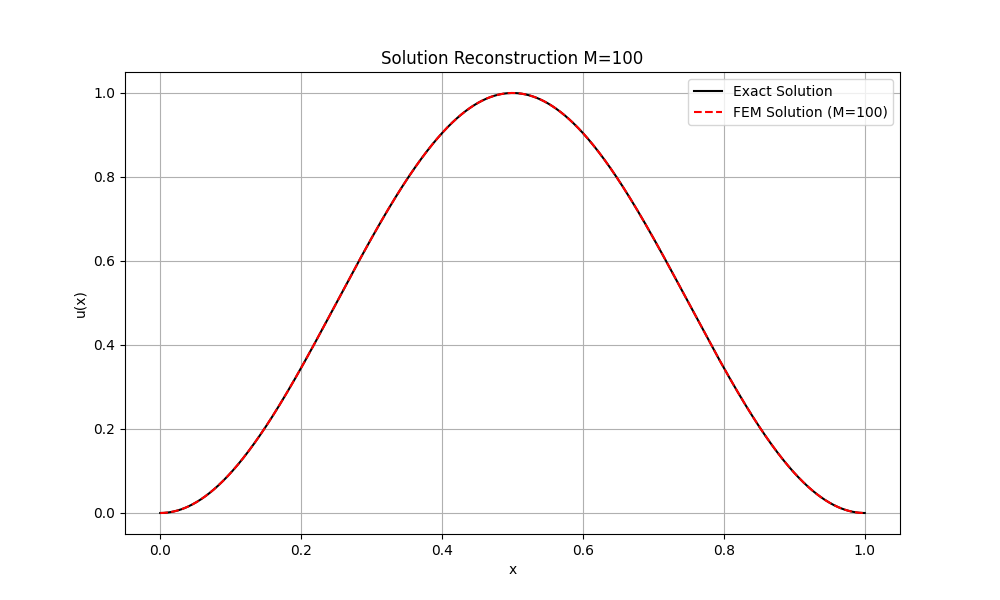
\includegraphics[width=0.8\textwidth]{solution.png}
    \caption{Finite element and analytic solution}
\end{figure}

\begin{figure}
    \centering
    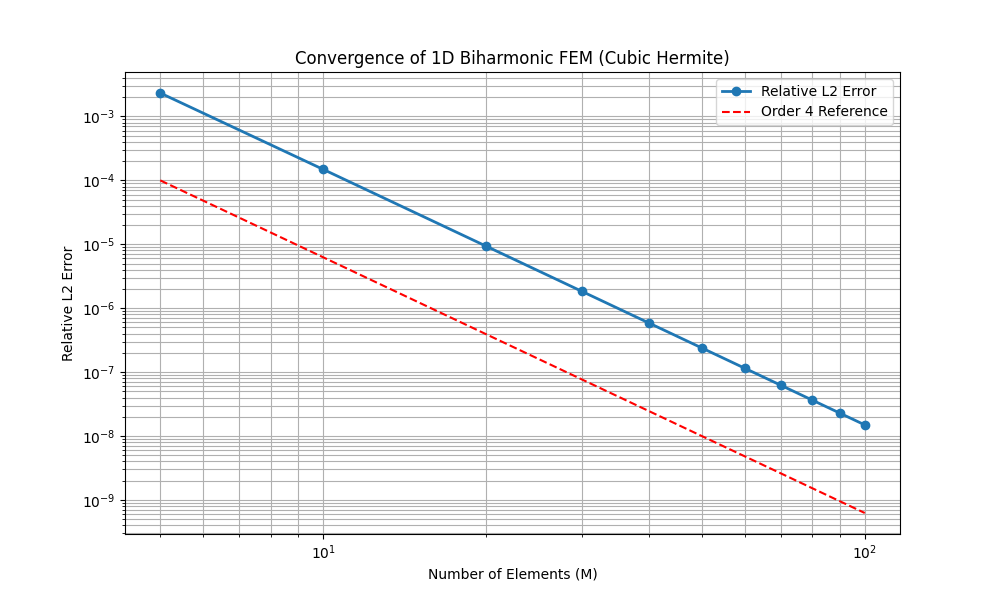
\includegraphics[width=0.8\textwidth]{convergence.png}
    \caption{Convergence Results}
\end{figure}



\clearpage
\section{Code}

\subsection{Gemini Response}

This code solves the 1D biharmonic equation $u^{(4)} = f$ (which corresponds to the weak form $\langle u'', v'' \rangle = \langle f, v \rangle$) with clamped boundary conditions $u(0)=u'(0)=u(1)=u'(1)=0$ using cubic Hermite Finite 




\begin{minted}[fontsize=\small]{python}
import numpy as np
import scipy.integrate as integrate
import scipy.sparse as sparse
import scipy.sparse.linalg as spla
import matplotlib.pyplot as plt

# ==========================================
# Module 1: Basis Functions & Local Integration
# ==========================================

def phi_L(x, a, b):
    h = b - a
    t = (x - a) / h
    return 1 - 3*t**2 + 2*t**3

def phi_R(x, a, b):
    h = b - a
    t = (x - a) / h
    return 3*t**2 - 2*t**3

def psi_L(x, a, b):
    h = b - a
    t = (x - a) / h
    return h * (t - 2*t**2 + t**3)

def psi_R(x, a, b):
    h = b - a
    t = (x - a) / h
    return h * (t**3 - t**2)

# Second derivatives for Stiffness Matrix
def d2_phi_L(x, a, b):
    h = b - a
    t = (x - a) / h
    return (1/h**2) * (-6 + 12*t)

def d2_phi_R(x, a, b):
    h = b - a
    t = (x - a) / h
    return (1/h**2) * (6 - 12*t)

def d2_psi_L(x, a, b):
    h = b - a
    t = (x - a) / h
    return (1/h) * (-4 + 6*t)

def d2_psi_R(x, a, b):
    h = b - a
    t = (x - a) / h
    return (1/h) * (-2 + 6*t)

def get_local_stiffness(a, b):
    """
    Numerically integrates the local stiffness matrix components.
    K_ij = integral(basis_i'' * basis_j'') dx
    Basis order: [phi_L, psi_L, phi_R, psi_R] (Value_L, Slope_L, Value_R, Slope_R)
    """
    funcs = [d2_phi_L, d2_psi_L, d2_phi_R, d2_psi_R]
    n = 4
    K_local = np.zeros((n, n))
    
    # Using fixed order quadrature (Simpson's or Gauss) is efficient, 
    # but we use scipy.integrate.quad as requested for generality.
    for i in range(n):
        for j in range(n):
            integrand = lambda x: funcs[i](x, a, b) * funcs[j](x, a, b)
            val, _ = integrate.quad(integrand, a, b)
            K_local[i, j] = val
            
    return K_local

def get_local_load(f, a, b):
    """
    Numerically integrates <f, v> for the local element.
    F_i = integral(f(x) * basis_i(x)) dx
    """
    funcs = [phi_L, psi_L, phi_R, psi_R]
    F_local = np.zeros(4)
    
    for i in range(4):
        integrand = lambda x: f(x) * funcs[i](x, a, b)
        val, _ = integrate.quad(integrand, a, b)
        F_local[i] = val
        
    return F_local

# ==========================================
# Solution Object (Reconstruction)
# ==========================================

class FEMSolution:
    def __init__(self, mesh, u_coeffs):
        self.mesh = mesh
        self.u_coeffs = u_coeffs # [u0, u'0, u1, u'1, ..., uM, u'M]
        
    def __call__(self, x_eval):
        # Handle scalar or vector input
        if np.isscalar(x_eval):
            return self._eval_single(x_eval)
        else:
            return np.array([self._eval_single(x) for x in x_eval])
            
    def _eval_single(self, x):
        # Clamp to domain
        x = max(self.mesh[0], min(self.mesh[-1], x))
        
        # Find element index
        # This assumes uniform mesh for O(1) lookup, but searchsorted is safer
        idx = np.searchsorted(self.mesh, x) - 1
        if idx < 0: idx = 0
        if idx >= len(self.mesh) - 1: idx = len(self.mesh) - 2
        
        a = self.mesh[idx]
        b = self.mesh[idx+1]
        
        # Indices in global vector
        # Node idx has DOFs at 2*idx, 2*idx+1
        # Node idx+1 has DOFs at 2*(idx+1), 2*(idx+1)+1
        c1 = self.u_coeffs[2*idx]     # u_L
        c2 = self.u_coeffs[2*idx+1]   # u'_L (psi_L coeff)
        c3 = self.u_coeffs[2*(idx+1)] # u_R
        c4 = self.u_coeffs[2*(idx+1)+1] # u'_R (psi_R coeff)
        
        val = (c1 * phi_L(x, a, b) + 
               c2 * psi_L(x, a, b) + 
               c3 * phi_R(x, a, b) + 
               c4 * psi_R(x, a, b))
        return val

# ==========================================
# Main Solver Class
# ==========================================

class BiharmonicSolver:
    def __init__(self, M, f_func=None):
        """
        M: Number of divisions (intervals)
        f_func: function f(x). If None, defaults to 0.
        """
        self.M = M
        self.f_func = f_func if f_func is not None else lambda x: 0.0
        self.mesh = np.linspace(0, 1, M + 1)
        self.n_nodes = M + 1
        self.n_dofs = 2 * self.n_nodes
        
    def assemble(self):
        # 2. Construct Stiffness Matrix A
        # 3. Construct Load Vector b
        
        # We use lil_matrix for efficient incremental construction
        A = sparse.lil_matrix((self.n_dofs, self.n_dofs))
        b = np.zeros(self.n_dofs)
        
        # Precompute local stiffness for a standard element (uniform grid)
        # Optimization: compute once since grid is uniform
        h = 1.0 / self.M
        K_local = get_local_stiffness(0, h)
        
        for e in range(self.M):
            x_L = self.mesh[e]
            x_R = self.mesh[e+1]
            
            # Map local indices [0,1,2,3] to global indices
            # Node L (index e): DOFs 2e, 2e+1
            # Node R (index e+1): DOFs 2(e+1), 2(e+1)+1
            indices = [2*e, 2*e+1, 2*(e+1), 2*(e+1)+1]
            
            # Add stiffness (Since uniform grid, K_local is valid for all elements 
            # if we ignore the x-shift in integration, which is valid for derivatives)
            # However, strict numerical integration of basis'' was requested. 
            # Note: The derivatives d2_phi depend on h, not absolute x.
            # So K_local is identical for all elements of size h.
            
            for i in range(4):
                for j in range(4):
                    A[indices[i], indices[j]] += K_local[i, j]
            
            # Load vector must be computed per element because f(x) varies
            F_local = get_local_load(self.f_func, x_L, x_R)
            for i in range(4):
                b[indices[i]] += F_local[i]
                
        self.A_full = A
        self.b_full = b
        
    def solve(self):
        # Apply Boundary Conditions
        # u(0)=0, u'(0)=0  => DOFs 0, 1
        # u(1)=0, u'(1)=0  => DOFs 2M, 2M+1
        
        bc_indices = [0, 1, 2*self.M, 2*self.M + 1]
        
        # Method: Penalty or Row/Col elimination. 
        # We will use Row/Col elimination (Identity trick) to keep matrix size
        # or simply slice the matrix for free DOFs. Slicing is cleaner for GMRES.
        
        free_indices = [i for i in range(self.n_dofs) if i not in bc_indices]
        
        A_free = self.A_full[free_indices, :][:, free_indices].tocsr()
        b_free = self.b_full[free_indices]
        
        # 4. Solve using GMRES
        # u_free, exit_code = spla.gmres(A_free, b_free, rtol=1e-6, restart=10, maxiter=300)
        u_free = spla.spsolve(A_free, b_free)
        
        # if exit_code != 0:
        #     print(f"GMRES did not converge for M={self.M}")
            
        # Reconstruct full vector
        u_full = np.zeros(self.n_dofs)
        u_full[free_indices] = u_free
        # Fixed DOFs remain 0
        
        return FEMSolution(self.mesh, u_full)

# ==========================================
# 5. Error Analysis & Plotting
# ==========================================

def run_analysis():
    # To demonstrate convergence, we need a non-zero analytic solution.
    # We choose the clamped beam solution: u(x) = x^2 * (1-x)^2 = x^2 - 2x^3 + x^4
    # This satisfies u(0)=u'(0)=u(1)=u'(1)=0.
    # u'' = 2 - 12x + 12x^2
    # u'''' = 24
    # So f(x) = 24.
    
    def u_exact(x):
        return np.sin(np.pi * x)**2
    
    def f_source(x):
        return -8*np.pi**4 *np.cos(2*np.pi*x)
    
    # If the user strictly wants f=0 as requested in the final line:
    # f_source = lambda x: 0.0
    # u_exact = lambda x: 0.0
    # (But this results in 0 error and empty plots, so we use the manufactured solution
    # to show the code capability as implied by "see the error decrease")
    
    Ms = [5, 10, 20, 30, 40, 50, 60, 70, 80, 90, 100]
    errors = []
    
    print(f"{'M':<5} | {'Relative L2 Error':<20}")
    print("-" * 30)
    
    for M in Ms:
        solver = BiharmonicSolver(M, f_source)
        solver.assemble()
        fem_sol = solver.solve()
        
        # Compute L2 Error
        # integral (u_fem - u_exact)^2 dx
        # We sum integrals over elements
        sq_err = 0.0
        norm_exact_sq = 0.0
        
        for i in range(M):
            a = solver.mesh[i]
            b = solver.mesh[i+1]
            
            # Integration for error
            integrand_err = lambda x: (fem_sol(x) - u_exact(x))**2
            val, _ = integrate.quad(integrand_err, a, b)
            sq_err += val
            
            # Integration for exact norm
            integrand_norm = lambda x: u_exact(x)**2
            val_norm, _ = integrate.quad(integrand_norm, a, b)
            norm_exact_sq += val_norm
            
        l2_err = np.sqrt(sq_err) / np.sqrt(norm_exact_sq)
        errors.append(l2_err)
        print(f"{M:<5} | {l2_err:.6e}")

    # Plotting
    plt.figure(figsize=(10, 6))
    plt.loglog(Ms, errors, 'o-', linewidth=2, label='Relative L2 Error')
    
    # Add reference slope lines (Expect O(h^4) or O(h^2) depending on norm)
    # H2 norm error for cubic is O(h^2), L2 should be O(h^4)
    h_vals = 1.0 / np.array(Ms)
    plt.loglog(Ms, 1e-4 * (np.array(Ms)/5.0)**(-4), 'r--', label='Order 4 Reference')
    
    plt.xlabel('Number of Elements (M)')
    plt.ylabel('Relative L2 Error')
    plt.title('Convergence of 1D Biharmonic FEM (Cubic Hermite)')
    plt.grid(True, which="both", ls="-")
    plt.legend()
    plt.show()
    plt.savefig("convergence.png")
    
    # Plot final solution comparison
    x_fine = np.linspace(0, 1, 1000)
    plt.figure(figsize=(10, 6))
    plt.plot(x_fine, u_exact(x_fine), 'k-', label='Exact Solution')
    plt.plot(x_fine, fem_sol(x_fine), 'r--', label=f'FEM Solution (M={Ms[-1]})')
    plt.xlabel('x')
    plt.ylabel('u(x)')
    plt.title(f'Solution Reconstruction M={Ms[-1]}')
    plt.legend()
    plt.grid()
    plt.show()
    plt.savefig("solution.png")

if __name__ == "__main__":
    # Module 0: Preliminary setup implicitly handled in run_analysis
    run_analysis()
\end{minted}




\end{document}
